\documentclass[a4paper,norsk]{article}
\usepackage[latin1]{inputenc}
\usepackage[T1]{fontenc}
\usepackage{babel,textcomp,listings, subfigure,graphicx}
\usepackage{subfig}

                                    
\title{Taylor Green vortex}
\author{Sebastian Gjertsen}
\begin{document}
\maketitle
\section*{Intro}
The Taylor Green vortex problem is a problem in fluid mechanics which details a cube with starting vortices, turning into turbulent flow and then decaying. To solve this problem I use the incompressible Navier-Stokes equations, and calculate the kinetic energy and compare with previous known results.


\section*{Problem definition}
I calculated the flow using a cube with sides $2\pi$. \newline
We have an initial distribution of velocity $\bar{u} = (u,v,w)$:
$$  u(x,y,z) = V_0sin(x)cos(y)cos(z) $$
$$  v(x,y,z) = - V_0cos(x)sin(y)cos(z)  $$
$$  w(x,y,z) = 0  $$
The Reynolds number is defined as: $Re = \frac{V_0 L}{\nu}$ where we set $V_0 = 1$



\section{Results}
These plots are of the kinetic energy and the negative time derivative of the kinetic energy. With N = 20, $\Delta t = 0.01, \nu = 5*10^{-3}$, giving $ Re = 1256  $.

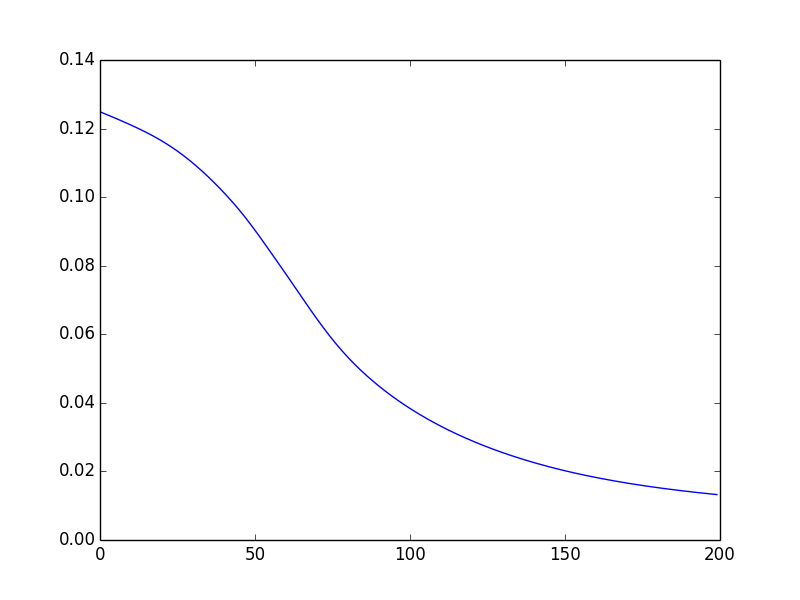
\includegraphics[trim = 0mm 0mm 0mm 0mm, clip, scale=0.4]{kinetic_e_best.png} 
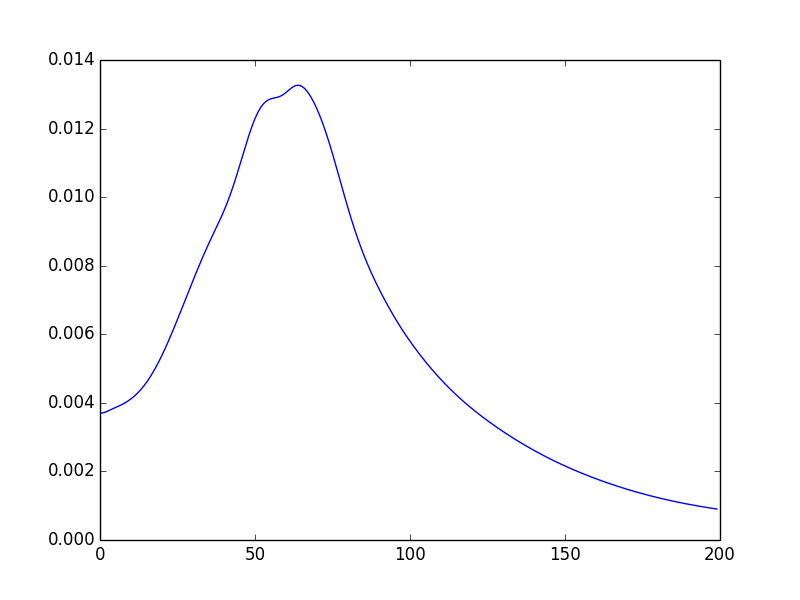
\includegraphics[trim = 0mm 0mm 0mm 0mm, clip, scale=0.4]{dKdt_best.png} 




\end{document}